\subsection{Modulos Arduino}
	\par 
		Los módulos de Arduino son esencialmente placas de circuitos independientes que integran uno o multiples circuitos integrados, sensores, pantallas LCD, componentes electronicos (capacitores, resistencias, inductores) y una interfaz de pines para una comunicación sencilla con la placa Arduino. Los modulos nos permiten agregar funcionalidad a nuestra placa arduino y son como piezas de un rompecabezas donde el resultado final es el prototipo deseado.
	
	\subsubsection{HC-05 (ZS-040)} 
		\par 
			El módulo HC-05 es un módulo Bluetooth SPP (Serial Port Protocol por sus siglas en ingles) fácil de usar, diseñado para la configuración de conexión en serie inalámbrica transparente. El módulo Bluetooth HC-05 se puede utilizar en una configuración maestra o esclava, lo que la convierte en una excelente solución para la comunicación inalámbrica .Este puerto en serie del módulo bluetooth es completamente calificado Bluetooth V2.0 + EDR (Enhanced Data Rate) Modulación de 3Mbps con un completo transceptor de radio de 2.4GHz y banda de base. 
	
		\begin{figure}[h]
			\centering
			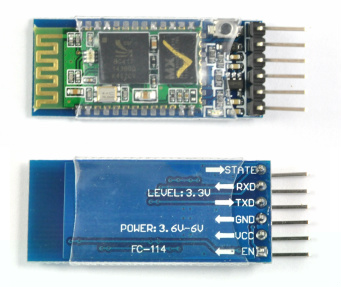
\includegraphics[width=8cm, height=6cm]{HC-05.jpg}
			\caption{}
		\end{figure}
	
\clearpage
\thispagestyle{plain}
	
	\subsubsection{nRF24L01}
		\par 
			El nRF24L01+ es un transceptor de 2.4GHz de un solo chip con un motor de protocolo de banda base integrado
			, adecuado para aplicaciones inalámbricas de muy baja potencia. El nRF24L01 + está diseñado
			para el funcionamiento en la banda de frecuencia ISM mundial a 2.400 - 2.4835GHz.
			
		\begin{figure}[h]
			\centering
			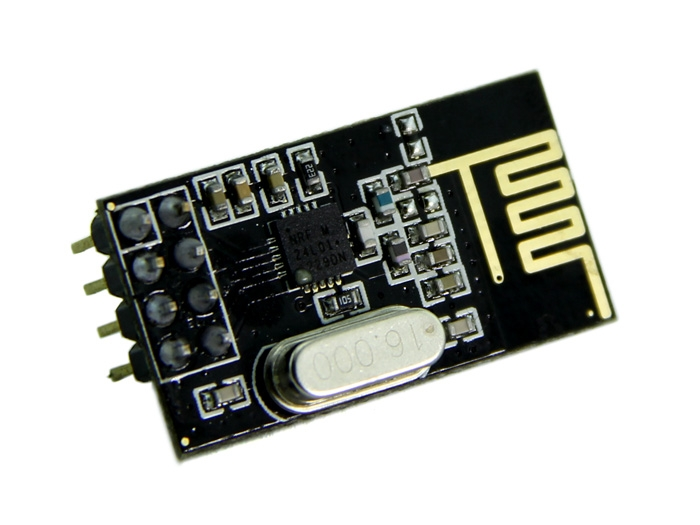
\includegraphics[width=8cm, height=6cm]{nrf24l01.jpg}
			\caption{}
		\end{figure}
			
		\par 
			Para diseñar un sistema de radio con nRF24L01 +, simplemente necesita una MCU (microcontrolador) y algunos componentes externos pasivos.
			
		\par 
			Se puede operar y configurar el nRF24L01 + a través de una interfaz de periféricos en serie (SPI). El registro
			mapa, que es accesible a través del SPI, contiene todos los registros de configuración en el nRF24L01 + y es
			accesible en todos los modos de operación del chip.
			
		\par 
			El motor de protocolo de banda base integrado se basa en la comunicación por paquetes
			y es compatible con varios modos, desde la operación manual hasta la operación de protocolo autónomo avanzado. 
			Los FIFOs internos aseguran un flujo de datos sin problemas entre la interfaz de radio y la MCU del sistema. El motor mejorado reduce el costo del sistema mediante el manejo de todas las operaciones de capa de enlace de alta velocidad.
			
		\par 
			La interfaz de radio usa la modulación GFSK. Tiene parámetros configurables por el usuario como canal de frecuencia,
			potencia de salida y velocidad de datos del aire. nRF24L01+ admite una velocidad de datos de aire de 250 kbps, 1 Mbps y 2 Mbps.
			La alta velocidad de datos de aire combinada con dos modos de ahorro de energía hacen que el nRF24L01+ sea muy adecuado para ultra bajo
			diseños de energía.